Again, the concept of a low-loss transmission line is a more practical transmission line where $R\ll\omega L$, $G\ll\omega C $.

Let us now study the conditions for treating the transmission line as low-loss at a particular frequency, the variation of voltage and current along a transmission line, the concept of voltage standing wave ratio (VSWR)\index{voltage standing wave ratio}, the condition for full reflection at the load end, the relationship between $R_{\max}$ and VSWR and also the relationship between $R_{\min}$ and VSWR.

The propagation constant in equation~\eqref{eqn:lowlossgamma} given as follows states the conditions defined for a low-loss transmission line in terms of the primary constants (R, L, C and G) of the line.
\begin{equation}
\gamma = \frac{1}{2}R\sqrt{\frac{C}{L}} + \frac{G}{2}\sqrt{\frac{L}{C}} +\jmath\omega\sqrt{LC}
\label{eqn:lowlossgammalec5}
\end{equation}
To treat a line as a low-loss transmission line, one will have to express these conditions ($R\ll\omega L$ and $G\ll\omega C$) in terms of the secondary parameters ($\alpha$ and $\beta$) since these parameters are readily available on the datasheet. If we can establish a relationship between these parameters ($\alpha$ and $\beta $) for the low-loss nature of the line, then we can find out whether a particular line is low-loss at a particular frequency.

The attenuation constant as derived in equation~\eqref{eqn:lowlossalpha} is
\begin{equation}
\alpha = \frac{1}{2}R\sqrt{\frac{C}{L}} + \frac{1}{2}G\sqrt{\frac{L}{C}}	
\label{eqn:lowlossalphalec5}
\end{equation}
And the phase constant remains the same as that of lossless transmission line
\begin{equation}
\beta = \omega\sqrt{LC}
\end{equation}
Since we have expressed equation~\eqref{eqn:lowlossgammalec5} in terms of primary constants, let us find out under what condition the transmission line can be treated as low-loss.

To do this we further simplify equation~\eqref{eqn:lowlossalphalec5} such that,
\begin{align*}
\alpha &=\frac{1}{2}R\sqrt{\frac{C}{L}} + \frac{1}{2}G\sqrt{\frac{L}{C}}\\	
&= \frac{1}{2} R \sqrt{\frac{C}{L}} \sqrt{\frac{L}{L}} + \frac{1}{2} G \sqrt{\frac{L}{C}} \sqrt{\frac{C}{C}}\footnotemark\\
&= \frac{1}{2} R \sqrt{\frac{CL}{L^2}} + \frac{1}{2} G \sqrt{\frac{LC}{C^2}}\\
&= \frac{1}{2} \frac{R}{L} \sqrt{LC} + \frac{1}{2} \frac{G}{C} \sqrt{LC}\\
&= \frac{1}{2} \frac{R}{\omega L} \omega \sqrt{LC} + \frac{1}{2} \frac{G}{\omega C} \omega \sqrt{LC}\footnotemark\\
&= \frac{1}{2} \omega\sqrt{LC}\left(\frac{R}{\omega L} + \frac{G}{\omega C}\right)
\end{align*}
But $\beta = \omega \sqrt{LC}$, so
\begin{equation}
\alpha = \beta\frac{1}{2} \left(\frac{R}{\omega L} + \frac{G}{\omega C}\right)
\end{equation}
\footnotetext{
The numerator and denominator of the first term is multiplied by $\sqrt{\frac{L}{L}}$ and the second term by $\sqrt{\frac{C}{C}}$,
}
\footnotetext{
The numerator and denominator is multiplied by $\omega$
}
Recall that for low-loss, $R\ll\omega L$ and $G\ll\omega C$, thus
\[\frac{R}{\omega L} \ll 1\textnormal{ and }\frac{G}{\omega C} \ll 1\]
Therefore, $\frac{1}{2} \left(\frac{R}{\omega L} + \frac{G}{\omega C}\right) \ll 1$ and $\alpha = \beta \times \textnormal{something far smaller than 1}$.

Hence, for a low-loss transmission line, $\alpha \ll \beta$ where $\beta = \frac{2 \pi}{\lambda}$.
Considering a wave which travels a distance of one wavelength along the transmission line, its phase, $\beta$ becomes $2\pi$, that is, $\beta = 2 \pi$, then the amplitude of the wave varies by
\begin{equation*}
e^{-\alpha x} = e^{-\alpha\lambda}	
\end{equation*}
Where $\lambda = \frac{2\pi}{\beta}$
\begin{equation*}
e^{-\alpha x} = e^{-\alpha \dfrac{2 \pi}{\beta}}
\end{equation*}
Since for a low-loss transmission line $\alpha\ll\beta$, therefore the quantity $e^{-\alpha \frac{2 \pi}{\beta}} \approx 1$. Hence, amplitude reduction is very small as the original amplitude is close to the final amplitude. So, a line can be treated as a low-loss transmission line if the change in amplitude over one wavelength is negligibly small. Let negligibly small be 1 percent change from the original or starting amplitude. Then
\[\frac{\alpha 2 \pi}{\beta} \approx \frac{1}{100}, e^{-0.01} = 0.99005\textnormal{ of the initial value}\]
The wave amplitude only reduces by $1-0.99005=0.00995$ or 1 per cent. That means the wave amplitude only reduces by 1 per cent after a distance of 1 wavelength.

A line can be treated as a low-loss transmission line if $\alpha \ll \beta$ depending on the given frequency but if the frequency changes such that $\alpha \geq \beta$, the line cannot be treated as a low-loss transmission line.

\begin{exmp}
\subsubsection*{Analysis of a Low-Loss transmission line}\label{lec:lec5}
Let's say we have a transmission line with $L = 0.25\mu H/m$, ${C= 100pF/m}$, $G = 0$, what is the resistance of the transmission line so that the line can be treated as a low-loss transmission line given the frequency of operation as $100MHz$?

\subsubsection*{Solution}
\[L= 0.25\mu H/m,C= 100pF/m, G = 0\]

\begin{dmath*}
\beta = 2\pi f\sqrt{LC}
=2 \pi \times 10^8 \sqrt{(0.25 \times 10^{-6}) \times (100 \times 10^{-12})} = \pi rad/m
\end{dmath*}
For a low-loss transmission line, taking 1 percent of $\beta,
\alpha= \frac{1}{100}\beta = \frac{\pi}{100}$.

Also,
\begin{equation*}
\alpha = \beta\frac{1}{2} \left(\frac{R}{\omega L} + \frac{G}{\omega C}\right)
\end{equation*}
Given that, \(G=0\)
\begin{equation*}
\alpha = \beta\frac{1}{2} \left(\frac{R}{\omega L}\right)
\end{equation*}
Recall that $\beta = \omega\sqrt{LC} $, now we get:
\begin{dmath*}
\alpha = \frac{1}{2}\frac{R}{\omega L} \times \omega\sqrt{LC} = \frac{1}{2} R \sqrt \frac{LC}{L^{2}} = \frac{1}{2} R \sqrt \frac{C}{L}
\end{dmath*}
\begin{equation*}
\frac{\pi}{100} = \frac{1}{2} R \sqrt{\frac{100 \times 10^{(-12)}}{0.25 \times 10^{(-6)}}}
\end{equation*}
\begin{equation*}
R=\pi\Omega/m.
\end{equation*}
If $R \leq \pi\Omega/m$, the line is low-loss at $ f= 100MHz$. If the frequency changes, the line may not satisfy this low-loss condition, hence we have to check again.
\end{exmp}

Therefore, unless specifically told that a line is a lossy line, we are at liberty to treat the line as a lossless line since the phase constant as we have seen for lossy and lossless lines are the same. Also, the characteristics impedance of a low-loss line is almost real and the same as the characteristics impedance of a lossless line. Hence for all transmission line problems, we consider it lossless and thus, 
\begin{align*}
Z_0 = \sqrt{{\frac{\jmath\omega L}{\jmath\omega C}}} = \sqrt{\frac{L}{C}} = \textnormal{real}, \quad \quad \gamma= \jmath\beta = \jmath\omega\sqrt{LC}
\end{align*}

\section{Voltage And Current Variation on a Lossless Transmission Line}
Revisiting the general voltage and current expression of the transmission line with origin at the load point, we have:
\begin{align}
V = V^+ e^{- \gamma x} + V^- e^{\gamma x}
\label{eqn:voltagefromloadlec5}\\
I= \frac{V^+}{Z_0} e^{- \gamma x} - \frac{V^-}{Z_0} e^{\gamma x}
\label{eqn:currentfromloadlec5}
\end{align}
\begin{figure}[h]
\centering
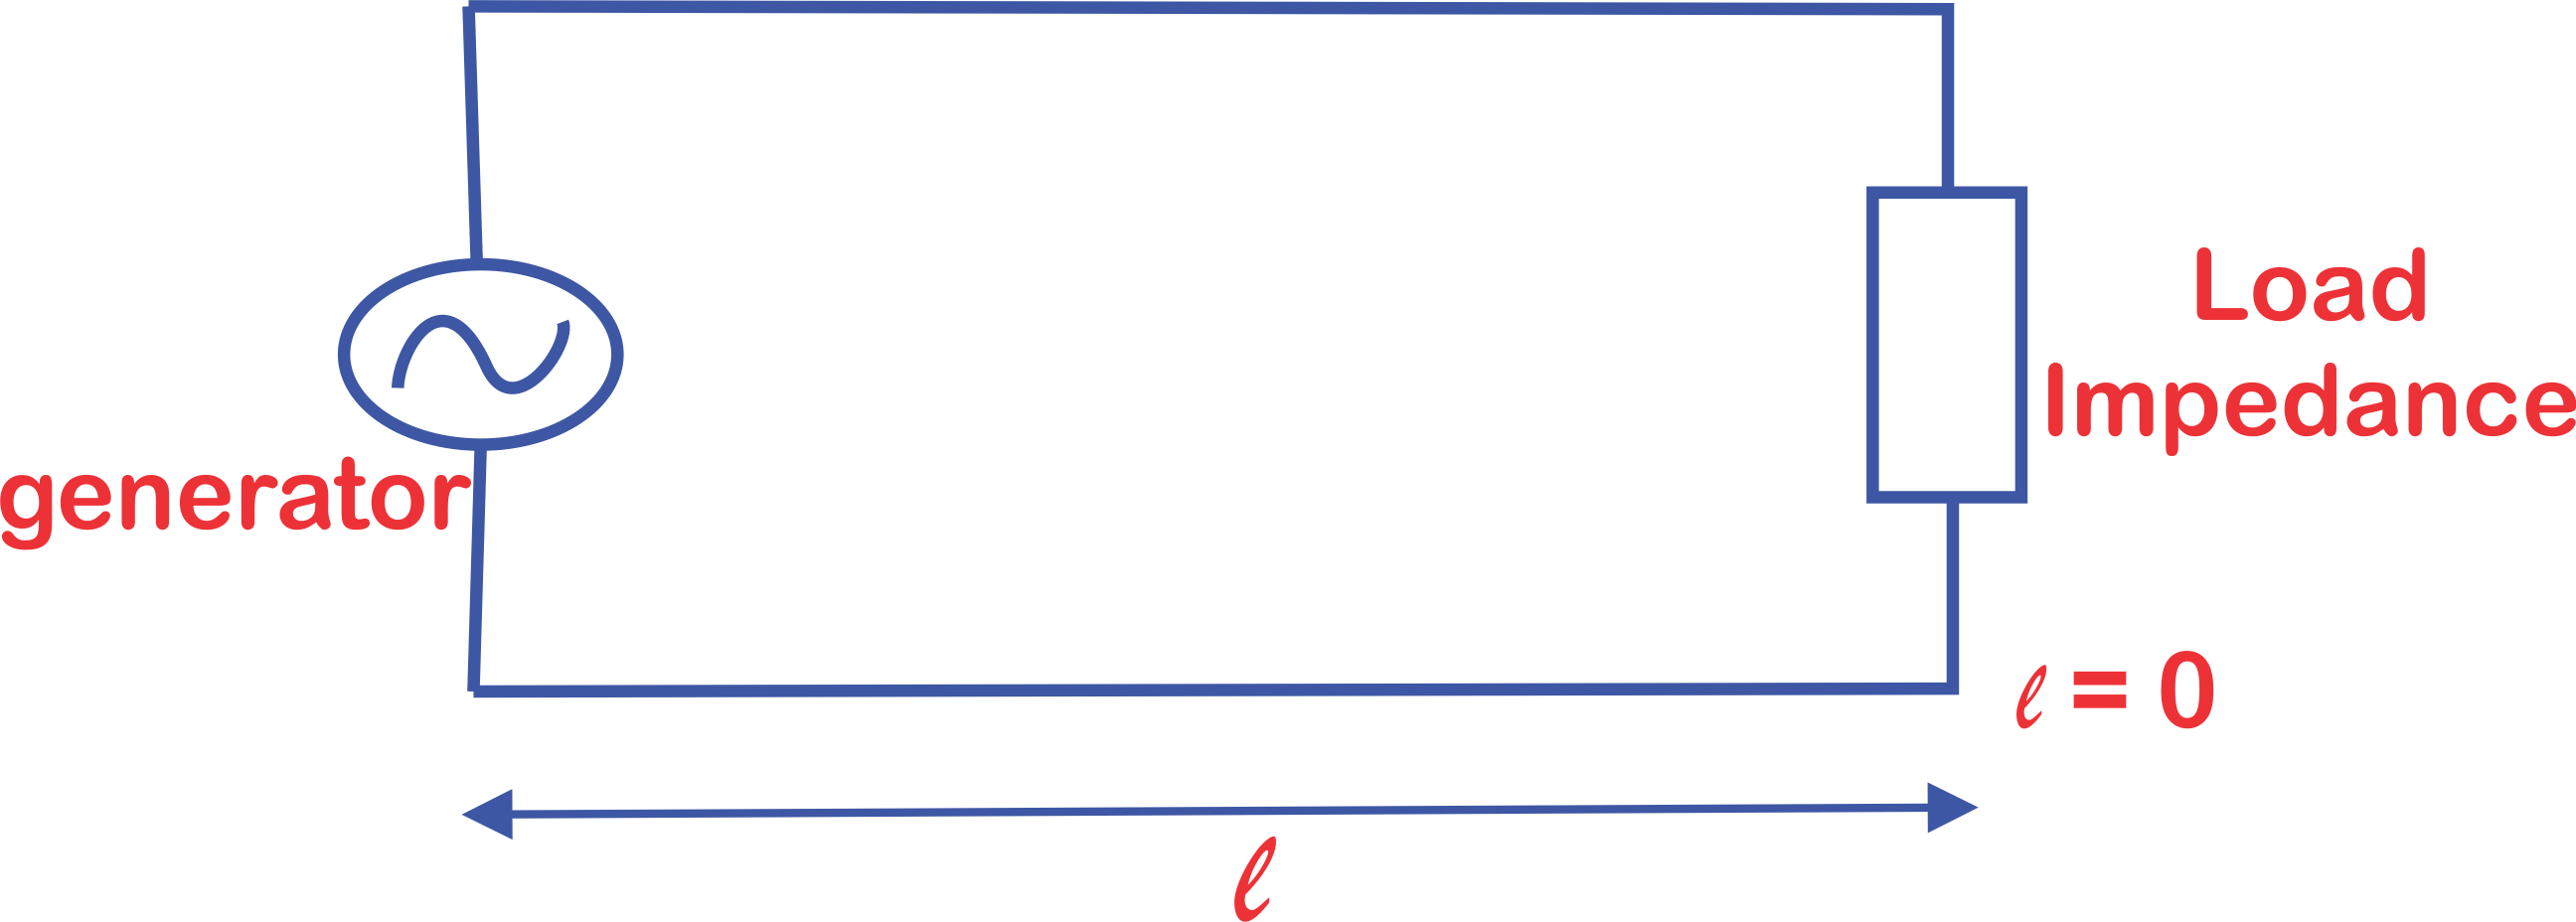
\includegraphics[width=0.9\linewidth]{./graphics/11111111}
\caption{Wave moving towards the Generator}
\label{fig:11111111}
\end{figure}

For a lossless transmission line at any point $l$, substituting $\gamma = \jmath\beta$ and $x=-l$ into equation~\eqref{eqn:voltagefromloadlec5}, we have;
\begin{align*}
V(l) &= V^+ e^{j \beta l} + V^- e^{-j\beta l}\\
\frac{V(l)}{ V^+ e^{j \beta l}} &= \left(1 +\frac{V^- e^{- j \beta l}}{V^+ e^{j \beta l}}\right)\footnotemark\\
V(l) &= V^+ e^{j \beta l}\left(1+ \frac{V^-}{V^+}e^{-j 2 \beta l}\right)
\end{align*}
\footnotetext{
The result is divided through by $ V^+ e^{j\beta l}$
}
Thus,
\begin{equation}
V(l) = V^+ e^{j \beta l}(1 + \Gamma_L e^{-j 2 \beta l})\quad\text{where }\Gamma _L = \frac{V^-}{V^+}
\label{eqn:voltagefromloadlossless}
\end{equation}

Similarly, substituting $\gamma = j\beta$ and $x = -l$ into equation~\ref{eqn:currentfromloadlec5}:
\begin{align*}
I(l) &= \frac{V^+}{Z_0} e^{\jmath \beta l} - \frac{V^-}{Z_0} e^{-\jmath\beta l}\\
\frac{I(l)}{\frac{V^+}{Z_0} e^{\jmath\beta l}} &= \left( 1- \frac{\frac{V^-}{Z_0} e^{-\jmath\beta l}}{\frac{V^+}{Z_0} e^{\jmath\beta l}}\right)\footnotemark\\
\frac{I(l)}{\frac{V^+}{Z_0} e^{\jmath\beta l}} &= \left(1- \frac{V^-}{V^+}e^{-\jmath 2 \beta l}\right)
\end{align*}
\footnotetext{
The result is divided through by $\frac{V^+}{Z_0} e^{\jmath\beta l}$
}
Thus,
\begin{equation}
I(l) = \frac{V^+}{Z_0}e ^{j \beta l} \left( 1 - \Gamma_L e^{-j 2 \beta l}\right)\quad\text{where }\Gamma _L = \frac{V^-}{V^+}
\label{eqn:currentfromloadlossless}
\end{equation}
From equations~\eqref{eqn:voltagefromloadlossless} and~\eqref{eqn:currentfromloadlossless}, $V = \mathfrak{f}( V^{+}, V^{-})$ and $I = \mathfrak{f}(I^{+}, I^{-})$ means $V$ and $I$ are a superposition of forward and backward travelling wave, which is then a \emph{standing wave}\index{standing wave}. Recall the reflection coefficient at the load end is given as
\begin{equation}
\Gamma_L = |\Gamma_L|e^{j\phi_L}
\label{eqn:refcoefficientfromload}
\end{equation}
where $\phi_L$ is the phase of the reflection coefficient at the load end. Then, we can write down the $V(l)$ and $I(l)$ explicitly in terms of the magnitude of the reflection coefficient and the phase.

Therefore substituting equation~\ref{eqn:refcoefficientfromload} into equations \ref{eqn:voltagefromloadlossless} and~\ref{eqn:currentfromloadlossless} respectively, we will get;
\begin{dmath}
V(l) = V^{+}e^{\jmath\beta l}(1 + |\Gamma_L|e^{j\phi_L} . e^{-j 2 \beta l})
= V^{+}e^{\jmath\beta l}(1 + |\Gamma_L| e^{\jmath(\phi_L -2 \beta l)})
\end{dmath}
And
\begin{dmath}
I(l) = \frac{V^+}{Z_0}e ^{j \beta l}( 1 - |\Gamma_L|e^{\jmath\phi_L} . e^{-\jmath 2\beta l})
= \frac{V^+}{Z_0}e ^{j \beta l}( 1 -|\Gamma_L| e^{j(\phi_L -2 \beta l)})
\end{dmath}
As we move from load to generator, $l$ increases positively, making $\phi_L -2\beta l$ more and more negative. In the complex plane, when a phase gets more negative, it means we are moving in a clockwise direction as shown in figure~\ref{fig:473-drawings}.
\begin{figure}[h]
\centering
\includegraphics[width=1\linewidth]{./graphics/"473 drawings"}
\caption{Clockwise and Anticlockwise movement of distance, $l$}
\label{fig:473-drawings}
\end{figure}

So by moving towards the generator, the phase becomes more and more negative, while the amplitude of $|\Gamma_L|$ remains constant. The total voltage is scaled by the vector sum of the real term (1) and complex term $|\Gamma_L| e^{j(\phi_L -2 \beta l)}$. Hence, we have a summation of a real vector, whose magnitude is 1, plus a complex term as shown in figure~\ref{fig:kjhgfdwert}. 
\begin{figure}[h]
\centering
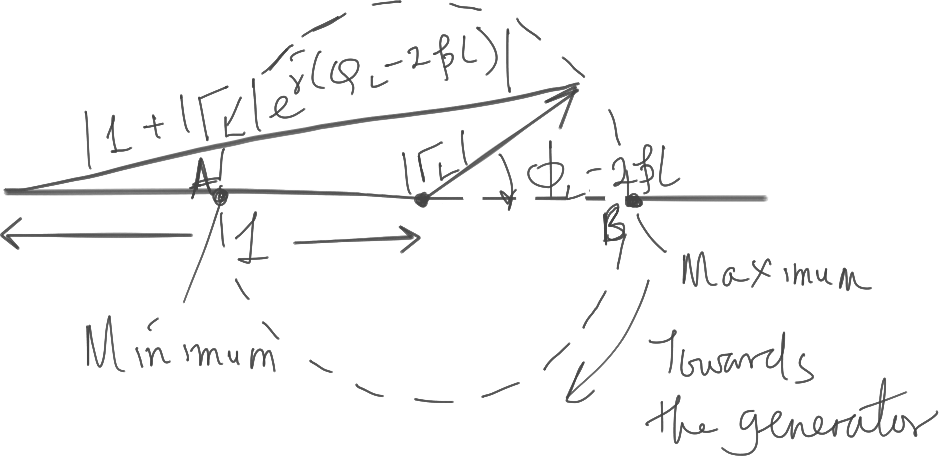
\includegraphics[width=0.8\linewidth]{./graphics/argand_diagram_temp}
\caption{Variation of the $1 + |\Gamma_L| e^{j(\phi_L -2 \beta l)}$ term in the complex plane (Argand diagram)}
\label{fig:kjhgfdwert}
\end{figure}

The magnitude $1+|\Gamma_L| e^{j(\phi_L -2 \beta l)}$ varies as we move along the transmission line.

From the \footnote{
Argand Diagram refers to a geometric plot of complex numbers as points $z = x + iy$ using the x-axis as the real axis and the y-axis as the imaginary axis. Such plots are named after Jean-Robert Argand (1768-1822), although they were first described by Norwegian-Danish land surveyor and mathematician Casper Wessel (1745-1818.)
}Argand diagram in figure~\ref{fig:kjhgfdwert}, the dash line circle is the variation plot of the term $\lvert\Gamma_L\rvert e^{j (\phi_L - 2\beta l)}$ whose magnitude is $\lvert \Gamma_L\rvert$ and phase $\phi_L - 2 \beta l$. The term $\lvert 1 + \lvert\Gamma_L\rvert e^{j (\phi_L - 2\beta l)}\rvert$ is the resolved vector of vector $1$ and vector $\lvert\Gamma_L\rvert e^{j (\phi_L - 2\beta l)}$. The same Argand diagram can be developed for the term $\lvert1 - \lvert\Gamma_L\rvert e^{j (\phi_L - 2\beta l)}\rvert$ where the vector $\lvert\Gamma_L\rvert e^{j (\phi_L - 2\beta l)}$ points in the negative direction. 

For even multiples of $\pi$, that is, $2n\pi$ where n is a positive integer then $\phi_L - 2\beta l = 2n\pi$ and $ e^{j(\phi_L - 2 \beta l)} = 1$. This is the maximum value of the resolved vector, that is, $1 + \lvert\Gamma_L\rvert$ and corresponds to point B in figure~\ref{fig:kjhgfdwert}.

For odd multiples of $\pi$, that is, $(2n + 1)\pi$, then $\phi_L - 2 \beta l=(2 n + 1)\pi$ and $e^{j (\phi_L - 2 \beta l)} = -1$. This is the minimum value of the resolved vector, that is, $1 - \lvert\Gamma_L\rvert$ and corresponds to point A in figure~\ref{fig:kjhgfdwert}. Similarly, $\lvert 1 - \lvert\Gamma_L\rvert e^{j (\phi_L - 2\beta l)}\rvert$ resolves to a maximum at odd multiples of $\pi$ and a minimum at even multiples of $\pi$.

Thus, $\lvert 1 + \lvert\Gamma_L\rvert e^{j (\phi_L - 2\beta l)}\rvert$ resolves to a maximum when $(\phi_L - 2\beta l) = 0, 2\pi, 4\pi, \ldots$ and $\lvert 1 + \lvert\Gamma_L\rvert e^{j (\phi_L - 2\beta l)}\rvert$ resolves to a minimum when $(\phi_L -2\beta l) = \pi, 3\pi, 5\pi \ldots$. This is the voltage term and implies the voltage is maximum when the phase equals even multiples of $\pi$ and minimum when the phase equals odd multiple of $\pi$.

This is opposite to the behaviour of the current relationship with the term $1-|\Gamma_L| e^{j(\phi_L -2\beta l)}$. At odd multiples of $\pi$ we have a maximum and at even multiples of $\pi$ we have a minimum.

Thus we have established that when $ e^{j(\phi_L - 2 \beta l)} = 1$, the voltage is maximum and the current is minimum and when $ e^{\jmath(\phi_L - 2 \beta l)} = -1$, the voltage is minimum and the current is maximum. So at the same location along the transmission line, maximum voltage corresponds to minimum current, and minimum voltage corresponds to maximum current. This is opposite to what we observed in a lumped circuit, where the maximum voltage point corresponds to maximum current and minimum voltage corresponds to minimum current.

The maximum voltage and current does not occur at the same point on the transmission line, they are staggered in space. Whenever there is a maximum voltage, there is a minimum current and vice versa. So the standing wave of voltage and current are shifted with respect to each other in space on the transmission line as shown in figure~\ref{fig:asdfghjhgfdsa}. 
\begin{figure}[h]
\centering
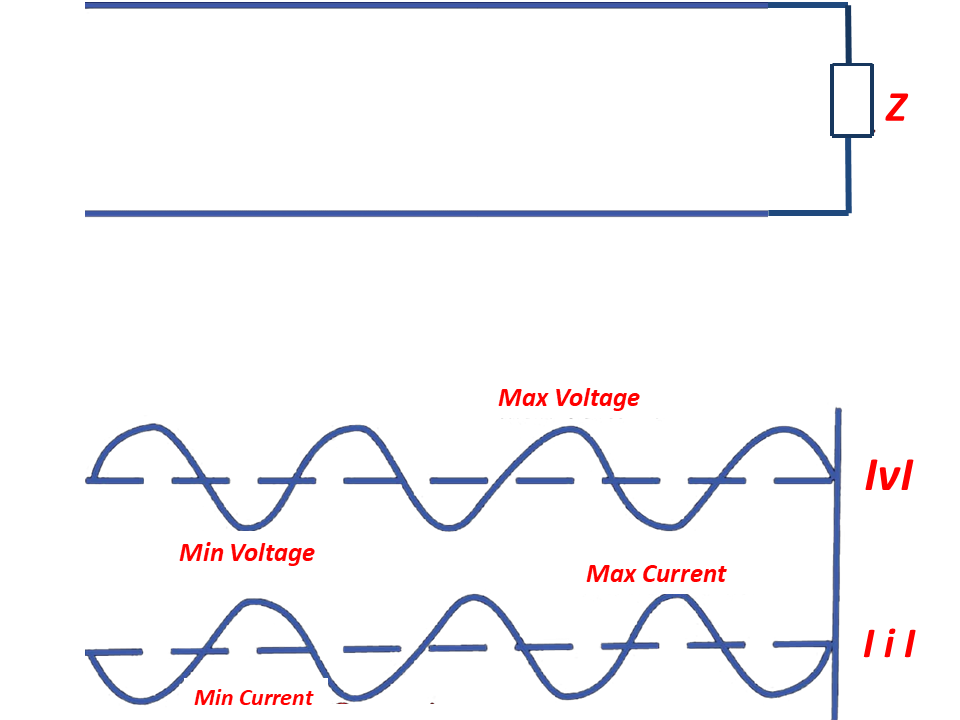
\includegraphics[width=0.7\linewidth]{./graphics/fig5.4modified}
\caption{Voltage and current variations for lossless transmission line in the direction of increasing $l$}
\label{fig:asdfghjhgfdsa}
\end{figure}

The plot of the voltage and current variations in figure~\ref{fig:asdfghjhgfdsa} shown that maximum voltage corresponds to minimum current and minimum voltage corresponds to maximum current.

\begin{exmp}
\subsubsection*{Maximum and Minimum voltage and current}
A lossless transmission line has 75$\Omega$ characteristic impedance. The line is terminated in a load impedance of $50-j100\Omega$. The maximum voltage measured on the line is 100V.

(a) Find the maximum and minimum current, and the minimum voltage on the line.

(b) At what distance from the load are the voltage and the current maximum?

\subsubsection*{Solution}
We are given
$Z_{0}=75\Omega$,
$Z_{L}=50-j100\Omega$, and 
$|V|_\max=100V$

\subsubsection*{(a) Maximum voltage and maximum and minimum current}
The first step is to calculate the reflection coefficient.
\begin{dmath*}
\Gamma_{L}=\frac{Z_{L}-Z_{0}}{Z_{L}+Z_{0}}
=\frac{50-j100-75}{50-j100+75}
=0.64\angle-65.3^o 
\end{dmath*}
Where $|\Gamma_{L}|=0.64$ and $\phi_{L}=-65.3^o$. Since we are told that the line is lossless, then the reflection coefficient will remain constant throughout the line.

We know that the maximum voltage which we will see on the line $|V|_\max=|V^{+}|(1+|\Gamma_{L}|)$, and we are given $|V|_\max$, we also know now the reflection coefficient, so we can find out the magnitude of the incident wave $|V^+|$.

So,
\begin{align*}
100&=|V^{+}|(1+0.64)\\
|V^{+}|&=\frac{100}{1.64}\\
&=60.8V
\end{align*}

Let us determine the maximum current and minimum voltage and current. Given the characteristic impedance and the maximum voltage, we can find the maximum current as 
\begin{align*}
|I|_\max&=\frac{|V|_\max}{Z_0}\\
&=\frac{100}{75}\\
&=1.33A
\end{align*}
The minimum current can be expressed in terms of minimum voltage as well so that
\begin{align*}
|I|_\min&=\frac{|V|_\min}{Z_0}\quad\text{But }|V|_\min\text{ = }|V^+|(1 - |\Gamma_L|)\\
&=\frac{|V^{+}|}{Z_0}(1-|\Gamma_{L}|)\\
&=\frac{60.8}{75}(1-0.64)\\
&=0.29A
\end{align*}
And we can determin the minimum voltage using either $|V|_\min=Z_0|I|_\min$ or $|V|_\min=|V^{+}|(1-|\Gamma_{L}|)$. Using the first equation, then the minimum voltage is	
\begin{dmath*}
|V|_\min=Z_0|I|_\min
=75\times0.29=21.88V
\end{dmath*}

\subsubsection*{(b) Location of maximum voltage and current}
Lastly, let us locate the distance from the load where the current and voltage are maximum. Let us note that when the two traveling waves have a constructive interference, we have a voltage maximum which corresponds to the current minimum. Also, when two traveling waves have a destructive interference, we have a voltage minimum which corresponds to the current maximum.

Recall that the phase difference between the forward and the backward wave is given by $\phi_{L}-2\beta l$. If $\phi_{L}-2\beta l$ equals even multiples of $\pi$, the two waves will  have a constructive interference and the voltage will be maximum. Similarly, when $\phi_{L}-2\beta l$ equals odd multiples of $\pi$, the two waves will have a destructive interference and a voltage minimal will be observed. So mathematically, voltage maximum occurs at $\phi_{L}-2\beta l= \pm2m\pi$, where m is an integer quantity.
\begin{align*}
\phi_{L}-2\beta l_\max&=-2m\pi\\
\text{Thus, }\quad2\beta l_\max&= \phi_{L}+2m\pi\\
\text{But, }\beta = \frac{2\pi}{\lambda}\\
2 \times \frac{2\pi}{\lambda}\times l_\max&= \phi_{L}+2m\pi\\
l_\max&=\frac{(\phi_L + 2m\pi)\lambda}{4\pi}
\end{align*}
We know $\phi_{L}=-65.3^o=-1.14rad$
\begin{align*}
l_\max=\frac{(-1.14 + 2m\pi)\lambda}{4\pi}
\end{align*}
When $m = 1,2,3, \ldots\quad l_\max=0.41\lambda, 0.91\lambda, 1.41\lambda$ and so on.

Similarly, to find the current maximum, let us recall that the current maximum occurs at a point where the voltage is minimum and vice versa. They are apart by a distance of $\frac{\lambda}{4}$, so the current maximum is at
\[
l_\max(\text{voltage})\pm \frac{\lambda}{4}
\]

Using the negative and positive sign will both give correct answers. Here, we will use the negative sign, that is, $l_\max-\frac{\lambda}{4}$. When $m = 1, 2, 3, \ldots$, therefore $|I|_\max$ occurs at $0.16\lambda , 0.66\lambda , 1.16\lambda$ and so on.
\end{exmp}

\section{Concept of Voltage Standing Wave Ratio (VSWR)}\index{voltage standing wave ratio}
Let us suppose we are interested in finding the impedance at an arbitrary distance $l$ on a lossless transmission line. Then the ratio of voltage and current would be
\begin{align*}
\frac{V(l)}{I(l)} = \frac{V^{+}e^{j\beta l}(1+ |\Gamma_L|e^{j(\phi_L- 2 \beta l)})}{\frac{V^{+}}{Z_0}(1- |\Gamma_L|e^{j(\phi_L- 2\beta l)})}
\end{align*}
Therefore,
\begin{equation*}
\frac{V(l)}{I(l)} = Z_0 \frac{1+ |\Gamma_L|e^{j(\phi_L- 2 \beta l)}}{1- |\Gamma_L|e^{j(\phi_L- 2\beta l)}}
\end{equation*}
For maximum voltage, $\phi_L-2\beta l = \textnormal{Even multiples of }\pi$ that is $0, 2\pi, 4\pi, 6\pi,\ldots$. For minimum voltage, $\phi_L-2\beta l=\textnormal{Odd multiples of } \pi$ that is $\pi, 3\pi,\ 5\pi,\ \ldots$. Thus the euler formular 
\[e^{j(\phi_L - 2 \beta l)} = \cos(\phi_L - 2 \beta l) + jsin(\phi_L - 2 \beta l)\]
Since $\sin(\phi_L - 2 \beta l) = 0$ for all multiples of $\pi$ or $n\pi$, where n is positive integer, therefore the euler relation is real. So when a voltage is maximum or minimum, $\frac{V(l)}{I(l)} = Z_0 \times$ (real quantity).

So irrespective of what the line is terminated with, at maximum voltage, the impedance at that point is always real. Even if the line is terminated with a complex impedance, the maximum voltage is always real. If we move to the point of maximum voltage, the impedance that will be measured at that point will always be real. Similarly, at the location where the voltage is minimum, the impedance will again be real.

In conclusion, on a transmission line, wherever there is a maximum voltage the impedance measured at that point will be real, same for the point of minimum voltage.

Mathematically, the maximum impedance is expressed as
\begin{dmath}
Z_{\max} = \frac{|V_{\max}|}{|I_{\min}|} 
= R_{\max}
= Z_0\left\{\frac{1+|\Gamma_L|}{1-|\Gamma_L|}\right\}
\label{eqn:maximp}
\end{dmath}
Similarly, at the location of minimum voltage, the minimum impedance is expressed as
\begin{dmath}
Z_{\min}=\frac{|V_{\min}|}{|I_{\max}|} 
= R_{\min}=Z_0\left\{\frac{1-|\Gamma_L|}{1+|\Gamma_L|} \right\}
\label{eqn:minimp}
\end{dmath}
Once load impedance, characteristic impedance $Z_0$ as well as the reflection coefficient $\Gamma_L$ are known, then we can calculate the maximum and minimum value of impedance that we see on the transmission line. As we move along the transmission line, the impedance will vary. However, there is a bound on the upper and lower value of this impedance; the lowest according to equation~\ref{eqn:maximp} and the lowest according to equation~\ref{eqn:minimp}.

At high frequencies, with the knowledge of the voltage standing wave on the transmission line, the measurement of phase is very difficult and complicated. One can measure the amplitude of a signal reliably but the measurement of phase is rather uncertain. So at high frequencies, we estimate the phase not in a direct manner but rather an indirect one by measuring only the magnitude quantities. As we have seen the phase of the signal in time gets translated into the space phase because the total phase we see on a wave is a combination of space and time relationship between the two waves, the forward and backward wave. 

These waves are related to the time phase and the space phase, $\omega t + \beta x$, where $\omega t$ is the temporal phase and $\beta x$ is the spatial phase. Since the total phase governs the location of maximum and minimum on the standing wave, noting the location of maximum and minimum on the transmission line, one can estimate the phase of the signal. Now we define a parameter for the standing wave which is a parameter of only amplitude variation of the transmission line. This quantity is called the \textbf{Voltage Standing Wave Ratio (VSWR)}\index{voltage standing wave ratio} \emph{which is the measure of the relative contribution of the reflected wave with respect to the incident wave}. If the reflected wave is zero, there is no standing wave but only a travelling wave and if the reflected wave is the same as the transmitted wave, then we have a completely developed standing wave. So the interference of the two waves, the forward and backward wave is going to give the variation of $R_{\max}$ to $R_{\min}$ and $R_{\min}$ to $R_{\max}$. So we define a quantity relating $V_{\max}$ and $V_{\min}$ as the VSWR.

Then 
\[\dfrac{V_{\max}}{V_{\min}}= VSWR, \rho\] 
VSWR is a very important quantity because without carrying out phase measurements, we can measure this quantity on a transmission line. Recall that the reflection coefficient is a complex quantity, so a complete knowledge of the reflection coefficient is achieved when both its amplitude and phase are known. However, the quantity which we are defining is known as VSWR or \(\rho\) which is measured only by amplitude.

Therefore, by measuring the maximum and minimum values of the standing wave, we get;
\begin{dmath*}
VSWR, \rho =\frac{|V|_{\max}}{|V|_{\min}} = \frac{|V^+|\{1+|\Gamma_L|\}}{|V^+|\{1-|\Gamma_L|\}}
\end{dmath*}
\begin{equation}
VSWR = \frac{1+|\Gamma_L|}{1-|\Gamma_L|}
\label{eqn:vswr}	
\end{equation}

\section{Condition for Full Reflection at Load End}
Since the transmission line is lossless, the reflection coefficient at the load is;
\begin{equation*}
|\Gamma_L| = \frac{Z_L-Z_0}{Z_L+Z_0}
\end{equation*}
Recall that $Z_0$ is real for a lossless transmission line and $Z_L$ can be any complex impedance as the load impedance. So, $|\Gamma_L| = \frac{Z_L-Z_0}{Z_L+Z_0}$ is always less than 1 that is:
\begin{equation*}
|\Gamma_L|\leq 1\quad (\textnormal{for a passive load})
\end{equation*}
What this means is that $|\Gamma_L|$ is the relative amplitude of the reflected wave with respect to the incident wave and its value no more than 1 implies that we do not have any energy source at the load point so the transmitted energy can only be reflected. Therefore, the amplitude of the reflected wave has to always be less than or equal to the amplitude of the incident wave.

\subsection{Conditions for which $|\Gamma_L|=1$}
\textbf{Case 1}: $Z_L=0$ (the line is short-circuited at the load end)
\begin{align*}	
\Gamma_L&= \frac{Z_L -Z_0}{Z_L + Z_0}\\
&= \frac{0 -Z_0}{0 + Z_0} = -1\\
\Rightarrow&|\Gamma_L|=1
\end{align*}	
\textbf{Case 2}: $Z_L=\infty$ (Open circuit line)
\begin{align*}
\Gamma_L&= \frac{Z_L -Z_0}{Z_L + Z_0}\\
&= \frac{1 -\frac{Z_0}{Z_L}}{1 + \frac{Z_0}{Z_L}} = \frac{1 - 0}{1 + 0} = 1\\
\Rightarrow&|\Gamma_L| = 1
\end{align*}
\textbf{Case 3}: $Z_L = \jmath X$ (Pure reactance)
\begin{align*}
\Gamma_L &= \frac{Z_L -Z_0}{Z_L + Z_0}\\
&= \frac{\jmath X - Z_0}{\jmath X + Z_0} = \textnormal{complex}\\
\Rightarrow&|\Gamma_L| = 1
\end{align*}
So the three cases under which $|\Gamma_L|=1$ are
\begin{enumerate}[(i)]
\item When the line is short-circuited.
\item When the line is open-circuited.
\item When the line is terminated in a pure reactance
\end{enumerate}
Since there is no energy-absorbing circuit at the load end of the line, short circuits, open circuits and ideal reactance cannot absorb power. So, whatever power the generator takes to the load end, it has no option but to return all the power in the reflected waveform.
\begin{align*}
VSWR = \frac{1+|\Gamma_L|}{1-|\Gamma_L|}
\end{align*}
The VSWR will always be greater than 1, the best case is $|\Gamma_L|=0$ (zero reflection) which gives $\rho=1$ whereas at $|\Gamma_L|=1$ (full reflection), $\rho= \infty$.

So $1\leq\rho\leq\infty$, where $\rho=1$ represents no reflected wave on the transmission line that is, full power is transferred to the load and $\rho = \infty$ means so much reflection on the transmission line or less efficiency of power transfer to the load. So, every circuit design tries to make VSWR as close to 1 as possible. A higher value of VSWR indicates more mismatch on the transmission line or a higher value of the reflected wave on the transmission line.

So VSWR is one of the most important quantities at high frequencies. When designing a circuit, we try to make sure the VSWR on the transmission line is close to one as possible, making sure the circuit is efficiently transferring power to the load end of the line. Once $\rho$ or VSWR is defined, we can relate it to the maximum and minimum impedance that can be seen on the transmission line.

\section{Maximum and Minimum Resistance}
From equations~\eqref{eqn:maximp} and~\eqref{eqn:minimp}, we can express the maximum and minimum impedance in terms of $\rho$\footnote{
Recall from equation~\eqref{eqn:vswr} that $\rho = \frac{1 + |\Gamma_L|}{1 - |\Gamma_L|}$
} such that
\begin{dmath}
R_{\max} = Z_0 \left(\frac{1 + |\Gamma_L|}{1 - |\Gamma_L|}\right)
= Z_0\rho
\label{eqn:maximprho}
\end{dmath}
\begin{dmath}
R_{\min} = Z_0 \left(\frac{1 - |\Gamma_L|}{1 + |\Gamma_L|}\right) 
=\frac{Z_0}{\rho}
\label{eqn:minimprho}
\end{dmath}
This implies that for any transmission line terminated with an arbitrary impedance, if we move to a point where the voltage is maximum or minimum, then we know the value of the impedance at that location. This is because with $V_{\max}$ and $V_{\min}$ known, we can determine $\rho$ and $Z_0$ is also known beforehand, hence $R_{\max}$ = $Z_0 \rho$ and $R_{\min} = \frac{Z_0}{\rho}$.

We know that the impedance known at any point in a transmission line can always be transformed to any other point using the impedance transformation relation. Hence knowing the location at voltage maximum or minimum, since the impedance value is known there, then we can transform the impedance value towards the load to get the load impedance. This essentially opens up a measurement technique for unknown impedance.

At high frequencies, if we have a complex impedance, its measurement is quite tedious because we cannot measure phase accurately. Now we have a mechanism for measuring the phase indirectly. As we have mentioned, the phase gets reflected into the standing wave pattern on the location of voltage maximum and minimum. So if we measure VSWR and the location of $V_{\max}$ and $V_{\min}$ we can always transform $R_{\max}$ or $R_{\min}$ to the location of the load which is nothing but the load impedance. So if we transform from the load impedance to the voltage maximum or minimum we would get $R_{\max}$ and $R_{\min}$. In summary, ig the location of $V_{\max}$ from the load is known and the value of impedance at that location, and the distance of the load from that point are also known, then the transformation of $R_{\max}$ or $R_{\min}$ to load end should give load impedance.


\begin{exmp}
\subsubsection*{Maximum and Minimum Resistance}
A $50\Omega$ transmission line is connected to a parallel combination of a $100\Omega$ resistance and a 1nF capacitance.

(a) Find the VSWR on the line at a frequency of 2MHz.

(b) Find the maximum and minimum resistance seen on the line.

\begin{figure}[h]
\centering
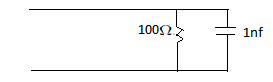
\includegraphics[width=\linewidth]{./graphics/d1}
\caption{Circuit diagram}
\end{figure}

\subsubsection*{Solution}
\begin{enumerate}[(i)]
\item First, we will find out the complete impedance for the parallel combination of the resistor and capacitor, given as $Z_{L}=R\parallel X_C$, that is
\begin{align*}
Z_L&=\frac{R \times X_c}{R + X_C}\quad\text{Where }X_C =\frac{1}{j\omega C}\\
&=\frac{R\times\dfrac{1}{j\omega C}}{\dfrac{j\omega RC + 1}{j\omega C}}\\
&=\frac{R}{j\omega C} \times \frac{j \omega C}{j\omega RC + 1}\\
&=\frac{R}{j\omega RC + 1}
\end{align*}
Given $f=2$MHz
\begin{dmath*}
\omega = 2\pi f
= 2\pi \times 2 \times 10^{6}
=1.256\times 10^{7}rad/s    
\end{dmath*}
Therefore the load impedance is
\begin{dmath*}
Z_{L}=\frac{100}{1 + j1.2566}
= 38.77-j48.7\Omega
= 62.3\angle-51.5^o\Omega
\end{dmath*}

\item Next, we find the refection coefficient.\\
Reflection coefficient at load point,
\begin{dmath*}
\Gamma_{L}=\frac{Z_{L}-Z_{0}}{Z_{L}+Z_{0}}
= \frac{38.77-j48.7-50}{38.77-j48.7+50}
=0.13-j0.47 = 0.5\angle-74.23^o
\end{dmath*}
We get $|\Gamma_{L}|=0.5$ and $\phi_L = -74.23^o$

\item 
\subsubsection*{(a) VSWR}
Now, we know the reflection coefficient, we can find out VSWR, $\rho$, given as;
\begin{dmath*}
\rho=\frac{1 + |\Gamma_{L}|}{1-|\Gamma_{L}|}=\frac{1+0.5}{1-0.5} = 3
\end{dmath*}

\item 
\subsubsection*{(b) Maximum and Minimum Resistance}
$R_\max$ and $R_\min$ can be calculated from equations~\eqref{eqn:maximprho} and~\eqref{eqn:minimprho} such that
\begin{align*}
R_\max = 50 \times 3 = 150\Omega\\
R_\min = \frac{50}{3} = 16.67\Omega
\end{align*}
\end{enumerate}
\end{exmp}

